\documentclass[10pt,aspectratio=169]{beamer}
\usepackage[T1]{fontenc}
\usepackage{helvet,booktabs,amsmath,tikz,pgfplots}
\pgfplotsset{compat=1.17,solid legend/.style={legend image code/.code={\draw[##1,draw=none] (0cm,-0.08cm) rectangle (0.25cm,0.14cm);}}}
\usetikzlibrary{arrows.meta,positioning}
\definecolor{ink}{HTML}{0B0B0B}
\definecolor{muted}{HTML}{52514E}
\definecolor{cnone}{HTML}{2A78D6}
\definecolor{cres}{HTML}{EB6834}
\definecolor{cgcn}{HTML}{1BAF7A}
\setbeamercolor{normal text}{fg=ink}
\setbeamercolor{frametitle}{fg=ink}
\setbeamercolor{title}{fg=ink}
\setbeamercolor{itemize item}{fg=muted}
\setbeamerfont{frametitle}{size=\large,series=\bfseries}
\setbeamerfont{title}{size=\Large,series=\bfseries}
\setbeamertemplate{navigation symbols}{}
\setbeamertemplate{itemize item}{\textbullet}
\setbeamertemplate{footline}{\hfill\color{muted}\scriptsize\insertframenumber\hspace{4mm}\vspace{3mm}}
\makeatletter\newcommand\rows[1]{\@@input ../generated/#1.tex }\makeatother
\tikzset{box/.style={draw=black!55,rounded corners=2pt,align=center,minimum height=10mm,inner xsep=6pt},
  arr/.style={-{Stealth[length=2mm]},black!65}}
\title{When Do Citations Help?}
\subtitle{A unified benchmark for scientific paper recommendation}
\author{PaperRec Project, IT4868E Web Mining}
\date{}
\begin{document}

\begin{frame}\titlepage\end{frame}

\begin{frame}{Two problems, one protocol}
\begin{itemize}\setlength\itemsep{3mm}
\item \textbf{Warm-start:} the paper already has saves. \textbf{Cold-start:} it has none.
\item CiteULike-a: 5,551 users, 16,980 papers, 204,986 saves, 44,661 citation links.
\item 13 methods on the same five folds, candidate pools and metrics.
\item Settings chosen on validation. Test used only for the final numbers.
\end{itemize}
\vspace{4mm}
\textbf{Question:} do citations add anything to a strong text encoder, and for which papers?
\end{frame}

\begin{frame}{Architecture}
\centering
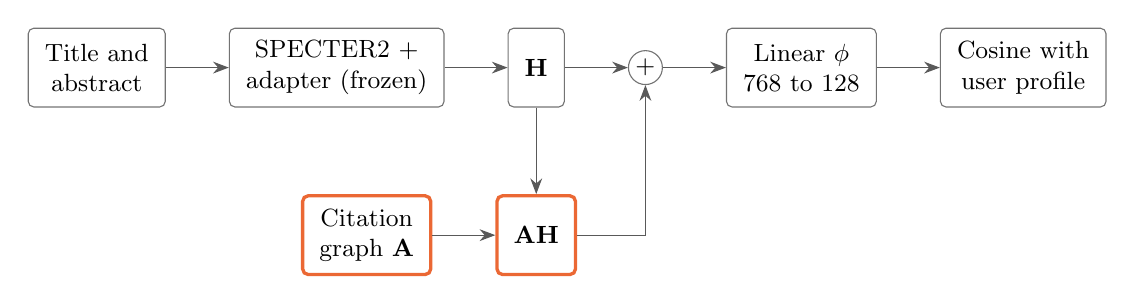
\begin{tikzpicture}[node distance=8mm and 8mm,font=\small]
\node[box] (text) {Title and\\abstract};
\node[box,right=of text] (enc) {SPECTER2 +\\adapter (frozen)};
\node[box,right=of enc] (h) {$\mathbf{H}$};
\node[circle,draw=black!55,right=of h,inner sep=1pt] (plus) {$+$};
\node[box,right=of plus] (phi) {Linear $\phi$\\768 to 128};
\node[box,right=of phi] (score) {Cosine with\\user profile};
\node[box,draw=cres,very thick,below=11mm of h] (ah) {$\mathbf{A}\mathbf{H}$};
\node[box,draw=cres,very thick,left=of ah] (cit) {Citation\\graph $\mathbf{A}$};
\draw[arr] (text)--(enc);\draw[arr] (enc)--(h);\draw[arr] (h)--(plus);\draw[arr] (plus)--(phi);\draw[arr] (phi)--(score);
\draw[arr] (h)--(ah);\draw[arr] (cit)--(ah);\draw[arr] (ah)-|(plus);
\end{tikzpicture}

\vspace{6mm}
\begin{tabular}{lll}
\texttt{nograph-bce} & $\phi(\mathbf{H})$ & control without citations\\
\texttt{gcn-bce} & $\phi(\mathbf{A}\mathbf{H})$ & plain GCN\\
\texttt{gcn-bce-add} & $\phi(\mathbf{H}+\mathbf{A}\mathbf{H})$ & residual GCN\\
\end{tabular}
\end{frame}

\begin{frame}{No leakage through the graph}
\centering
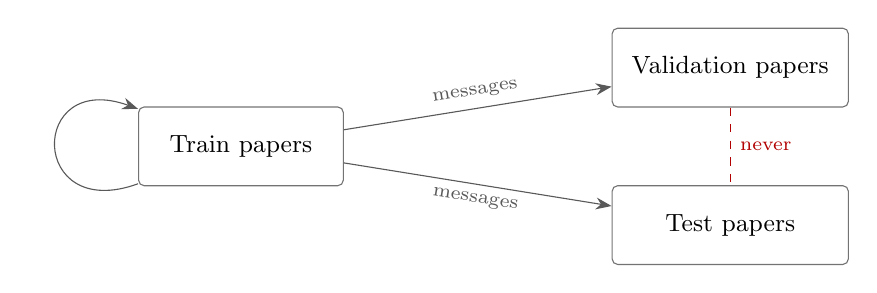
\begin{tikzpicture}[node distance=16mm,font=\small]
\node[box,minimum width=26mm] (tr) {Train papers};
\node[box,right=34mm of tr,yshift=10mm,minimum width=30mm] (va) {Validation papers};
\node[box,right=34mm of tr,yshift=-10mm,minimum width=30mm] (te) {Test papers};
\draw[arr] (tr)--node[above,sloped,font=\scriptsize]{messages}(va);
\draw[arr] (tr)--node[below,sloped,font=\scriptsize]{messages}(te);
\draw[arr] (tr) to[out=200,in=160,looseness=4] (tr);
\draw[dashed,red!70!black] (va)--node[right,font=\scriptsize]{never}(te);
\end{tikzpicture}

\vspace{6mm}
Held-out papers receive from training papers and send to nobody.\\
Training embeddings do not depend on held-out papers.
\end{frame}

\begin{frame}{Test results}
\centering\scriptsize
\begin{tabular}{lcccccc}
\toprule
 & \multicolumn{3}{c}{Warm-start} & \multicolumn{3}{c}{Cold-start}\\
Model & R@20 & NDCG@20 & MRR & R@20 & NDCG@20 & MRR\\
\midrule
\rows{overview}
\bottomrule
\end{tabular}

\vspace{1mm}
$\dagger$ no signal for unseen papers, so the cold ranking is random. Means over five folds.
\end{frame}

\begin{frame}{Where the gains come from}
\centering\scriptsize
\resizebox{\linewidth}{!}{%
\begin{tabular}{llcccccc}
\toprule
 & & \multicolumn{3}{c}{Recall@20} & \multicolumn{3}{c}{NDCG@20} \\
Setting & Comparison & Gap & 95\% interval & Folds & Gap & 95\% interval & Folds \\
\midrule
\rows{paired_test}
\bottomrule
\end{tabular}}

\normalsize\vspace{4mm}
\begin{itemize}
\item Training on saves gives most of the gain.
\item Citations hurt if they replace a paper's own features, and help if added to them.
\end{itemize}
\end{frame}

\begin{frame}{The cold-start gain reverses for uncited papers}
\centering
\begin{tikzpicture}
\begin{axis}[ybar=1.5pt,solid legend,ytick={0,0.1,0.2,0.3,0.4,0.5},bar width=11pt,width=0.92\linewidth,height=5.3cm,
  ymin=0,ymax=0.5,symbolic x coords={0,1,2--3,4--7,8+},xtick=data,enlarge x limits=0.13,
  xlabel={Citations visible at inference},ylabel={Hit rate@20},font=\small,
  axis lines*=left,tick style={draw=none},ymajorgrids,grid style={black!10},
  legend style={draw=none,at={(0.02,1.0)},anchor=north west,legend columns=3}]
\addplot[fill=cnone,draw=none] table[x=bucket,y=nograph]{../generated/cold_degree.dat};
\addplot[fill=cres,draw=none] table[x=bucket,y=residual]{../generated/cold_degree.dat};
\addplot[fill=cgcn,draw=none] table[x=bucket,y=plain]{../generated/cold_degree.dat};
\legend{No graph,Residual GCN,Plain GCN}
\end{axis}
\end{tikzpicture}

Residual minus no graph: $-0.066$ with no citations, $+0.117$ with eight or more.
\end{frame}

\begin{frame}{Why: exposure and direct links}
\centering\small
\begin{tabular}{lcccc}
\toprule
 & No & Cited, no link & One link & Two or more \\
Cold test hit rate@20 & citations & to profile & to profile & to profile \\
\midrule
\rows{cold_link}
\bottomrule
\end{tabular}

\vspace{4mm}
\begin{itemize}
\item Uncited papers are 35.4\% of the pool. They get 33.0\% of top-20 slots without the graph and 21.9\% with it.
\item Citations help mainly when they reach the user's own library.
\end{itemize}
\end{frame}

\begin{frame}{Takeaways}
\begin{itemize}\setlength\itemsep{3mm}
\item \textbf{Warm-start:} collaborative filtering wins (WMF 0.522 Recall@20, best citation model 0.415).
\item \textbf{Cold-start:} the residual GCN is best on average (0.400 against 0.387).
\item \textbf{New papers with no citations:} prefer \texttt{nograph-bce} (0.312 against 0.246 hit rate).
\end{itemize}
\vspace{5mm}
\textbf{Limits:} citations are undated, so cold scores of citation models are optimistic. One dataset, one test seed, unequal tuning. The causes of the uncited-paper loss are not established.
\end{frame}
\end{document}
